\section{Design}

\subsection{System Architecture}

As discussed during the planning stages, Choona will be built using the microservices architecture. Figure \ref{fig:architecture} shows the proposed system design of the Choona, split into four layers.

\begin{figure}[h!]
  \centering
  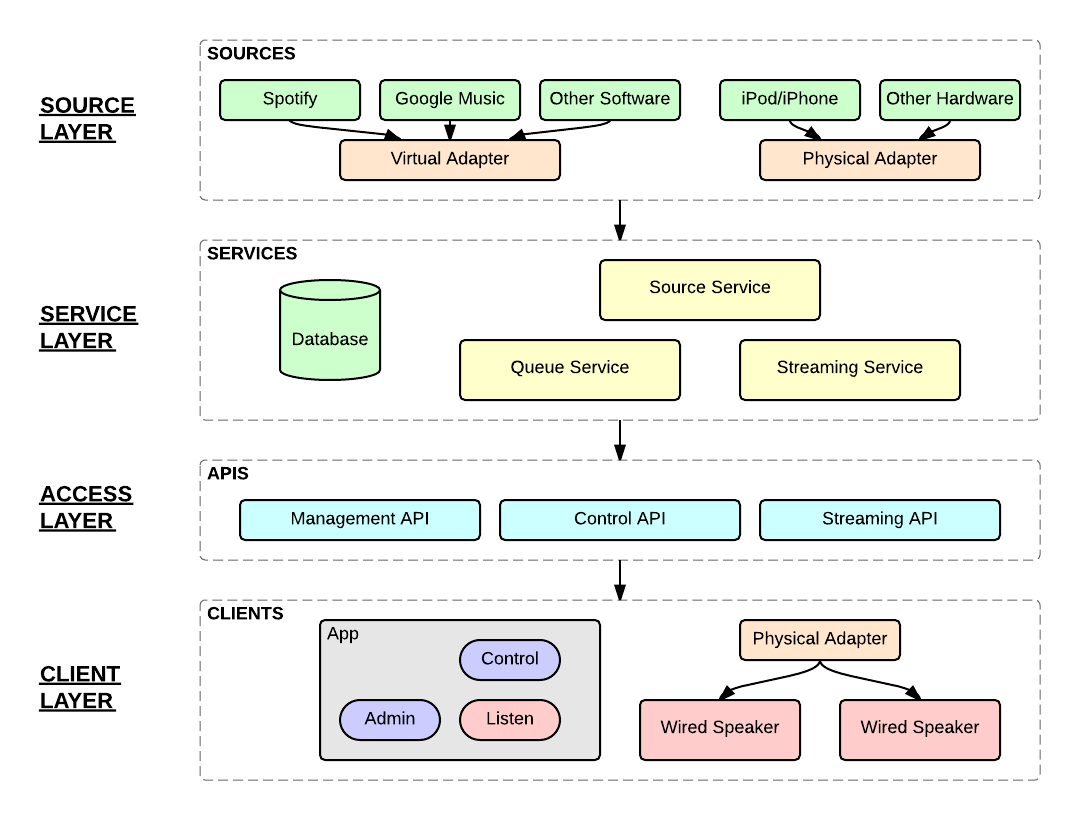
\includegraphics[width=1\textwidth]{./img/sys-architecture.png}
  \caption{Proposed Choona system architecture}
  \label{fig:architecture}
\end{figure}

\begin{itemize}
  \item \textbf{Source Layer}\\
    Sources, such as Spotify and Google Music, all have their own unique APIs. For them to be consumed by Choona they need to present a common interface otherwise other services will need to know how to interact directly with each individual API. Therefore each source will be exposed through either a virtual or physical adapter. Each adapter understands the same set of commands and outputs data in the same format. This means that other services in Choona only need to implement the standard adapter interface in order to communicate with any type of audio source. For the first version of Choona the sources will only need to understand a basic set of instructions:
    \begin{itemize}
      \item \texttt{search [searchString]} - search the source's track database using the supplied search string
      \item \texttt{get [trackId]} - retrieve track information from the source's database for the specified track ID
      \item \texttt{play [trackId]} - stream the audio for the specified track ID
    \end{itemize}

  \item \textbf{Service Layer}\\
    The service layer contains the majority of the \textit{business logic} of the Choona server-side infrastructure. There will be three main services at this layer. The queue service is responsible for maintaining the running playlist of tracks for a particular Choona location. The source service acts as an interface to all the different types of audio sources (instructions documented above). The streaming service takes tracks from the queue service, retrieves the audio via source service and sequences it into a single stream that the APIs can then send to clients. This layer has a more extensive set of instructions:
    \begin{itemize}
      \item \texttt{queue join [locationId] [clientId]} - make a client join a particular location
      \item \texttt{queue add [locationId] [trackId]} - add a song to the queue of a particular location
      \item \texttt{queue upvote [locationId] [trackId]} - upvote a song at a particular location
      \item \texttt{queue downvote [locationId] [trackId]} - upvote a song at a particular location
      \item \texttt{stream add [locationId] [trackId]} - instruct the streaming service to play a particular track next at a certain location
      \item \texttt{stream play [locationId]} - broadcast the stream to all listening clients of a location
    \end{itemize}

  \item \textbf{Access Layer}\\
    The access layer contains APIs that clients can use to interact with the Choona infrastructure. These APIs act as proxies, taking requests from clients and passing them through to the right services in the service layer. The only special instruction the access layer makes available is user authentication verification.

  \item \textbf{Client Layer}\\
    The client layer contains all the consumers of Choona, such as the mobile app and speaker adapter. Clients use the access layer to authenticate and interact with the rest of the Choona infrastructure; they do not need to know about all the individual services, instead they only need to understand the access APIs.
\end{itemize}